
% ----------------------------------------------------------------------
%  Set the document class
% ----------------------------------------------------------------------
\documentclass[11pt,a4paper,twoside]{article}

% ----------------------------------------------------------------------
% Define external packages, language, margins, fonts and new commands
% ----------------------------------------------------------------------
%\input{preamble} 
\usepackage[utf8]{inputenc}   % <<<<< Linux
\usepackage[english]{babel} % <<<<< English
\usepackage{notoccite}
\usepackage[skip=0.5\baselineskip]{caption}
\hyphenation{GTKWave}
\usepackage{listings}
\usepackage[all]{nowidow}

%blind text
\usepackage{lipsum}

\usepackage{graphicx}
\graphicspath{ {./} {../../figlib/} }
\def\FontLn{% 16 pt normal
  \usefont{T1}{phv}{m}{n}\fontsize{16pt}{16pt}\selectfont}
\def\FontLb{% 16 pt bold
  \usefont{T1}{phv}{b}{n}\fontsize{16pt}{16pt}\selectfont}
\def\FontMn{% 14 pt normal
  \usefont{T1}{phv}{m}{n}\fontsize{14pt}{14pt}\selectfont}
\def\FontMb{% 14 pt bold
  \usefont{T1}{phv}{b}{n}\fontsize{14pt}{14pt}\selectfont}
\def\FontSn{% 12 pt normal
  \usefont{T1}{phv}{m}{n}\fontsize{12pt}{12pt}\selectfont}

% Use Arial font as default
%
\renewcommand{\rmdefault}{phv}
\renewcommand{\sfdefault}{phv}
\usepackage{geometry}	
\geometry{verbose,tmargin=2.5cm,bmargin=2.5cm,lmargin=2.5cm,rmargin=2.5cm}

%\usepackage{setspace}
%\renewcommand{\baselinestretch}{1.5}

\usepackage[pdftex]{hyperref} % enhance documents that are to be
                              % output as HTML and PDF
\hypersetup{colorlinks,       % color text of links and anchors,
                              % eliminates borders around links
%            linkcolor=red,    % color for normal internal links
            linkcolor=black,  % color for normal internal links
            anchorcolor=black,% color for anchor text
%            citecolor=green,  % color for bibliographical citations
            citecolor=black,  % color for bibliographical citations
%            filecolor=magenta,% color for URLs which open local files
            filecolor=black,  % color for URLs which open local files
%            menucolor=red,    % color for Acrobat menu items
            menucolor=black,  % color for Acrobat menu items
%            pagecolor=red,    % color for links to other pages
            pagecolor=black,  % color for links to other pages
%            urlcolor=cyan,    % color for linked URLs
            urlcolor=black,   % color for linked URLs
	          bookmarks=true,         % create PDF bookmarks
	          bookmarksopen=false,    % don't expand bookmarks
	          bookmarksnumbered=true, % number bookmarks
	          pdftitle={report},
            pdfauthor={Andre C. Marta},
%            pdfsubject={Thesis Title},
%            pdfkeywords={Thesis Keywords},
            pdfstartview=FitV,
            pdfdisplaydoctitle=true}

\usepackage[numbers,sort&compress]{natbib} % <<<<< References in numbered list [1],[2],...
\usepackage{subcaption} 
\usepackage{mdframed}

%%%%%%%%%%%%%%%%%%%%%%%%%%%%%%%%%%%%%%%%%%%%%%%%%%%%%%%%%%%%%%%%%%%%%%%%
%     Begin Document                                                   %
%%%%%%%%%%%%%%%%%%%%%%%%%%%%%%%%%%%%%%%%%%%%%%%%%%%%%%%%%%%%%%%%%%%%%%%%


\begin{document}

% Set plain page style (no headers, footer with centered page number)
\pagestyle{plain}

% Set roman numbering (i,ii,...) before the start of chapters
%\pagenumbering{roman}

% ----------------------------------------------------------------------
%  Cover page
% ----------------------------------------------------------------------
%%%%%%%%%%%%%%%%%%%%%%%%%%%%%%%%%%%%%%%%%%%%%%%%%%%%%%%%%%%%%%%%%%%%%%%
%                                                                      %
%     File: Thesis_FrontCover.tex                                      %
%     Tex Master: Thesis.tex                                           %
%                                                                      %
%     Author: Andre C. Marta                                           %
%     Last modified :  2 Jul 2015                                      %
%                                                                      %
%%%%%%%%%%%%%%%%%%%%%%%%%%%%%%%%%%%%%%%%%%%%%%%%%%%%%%%%%%%%%%%%%%%%%%%%

\thispagestyle {empty}

% IST Logo - Signature A
% parameters: bb=llx lly urx ury (bounding box), width=h_length, height=v_length, angle=angle, scale=factor, clip=true/false, draft=true/false. 





\begin{center}
%\begin{figure}[h] \centering


% Figure (Image or plot)
\vspace{1.0cm}
% height = 50 mm
%\includegraphics[height=50mm]{Figures/Airbus_A350.jpg}

% Title, author and degree
\vspace{1cm}
{\FontLb Circuit Theory and Electronics Fundamentals} \\ % <<<<< EDIT TITLE
\vspace{1cm}
{\FontSn Instituto Superior Técnico, University of Lisbon} \\ % <<<<< EDIT COURSE
\vspace{1cm}

\begin{figure}[h] \centering
\includegraphics[width=0.8\linewidth]{IST_A_CMYK_POS} 
\end{figure}

{\FontSn Laboratory 2} \\
\vspace{1cm}
{\FontSn MeAer} \\
\vspace{1cm}
{\FontSn Dinis Salgado, 90560} \\
\vspace{0.5cm}
{\FontSn Bruno Santos, 98460} \\
\vspace{0.5cm}
{\FontSn Laura Cebola, 98464} \\
\vspace{1cm}
{\FontSn April 08, 2021} \\ % <<<<< EDIT DATE (corresponds to date of oral examination)
\vspace{1cm}
%
\end{center}



% ----------------------------------------------------------------------
% Dedication page (optional)
% ----------------------------------------------------------------------
%\input{dedication} 
%\cleardoublepage

% ----------------------------------------------------------------------
%  Acknowledgments (optional)
% ----------------------------------------------------------------------
%\input{acknowledgements}
%\cleardoublepage

% ----------------------------------------------------------------------
%  Abstract (both in English and Portuguese)
% ----------------------------------------------------------------------
%\input{resumo} 
%\cleardoublepage

%\input{abstract} 

% ----------------------------------------------------------------------
%  Table of contents, list of tables, list of figures and nomenclature
% ----------------------------------------------------------------------

% Table of contents
%
\tableofcontents

% List of tables
%\addcontentsline{toc}{section}{\listtablename}
%\listoftables
%\cleardoublepage 

% List of figures
%\addcontentsline{toc}{section}{\listfigurename}
%\listoffigures
%\cleardoublepage 

% Set arabic numbering (1,2,...) after preface
%
%\setcounter{page}{1}
%\pagenumbering{arabic}

% ----------------------------------------------------------------------
%  Body
% ----------------------------------------------------------------------

\newpage

\section{Introduction}
\label{sec:introduction}

% state the learning objective 
The objective of this laboratory assignment is to study a circuit containing a
sinusoidal voltage source $V_S$ connected to seven resistors, $R$, a dependent voltage source, $V_d$, a dependent current source $I_b$ and a capacitor $C$. The circuit can be seen in Figure~\ref{fig:rc}.


In Section~\ref{sec:analysis}, a theoretical analysis of the circuit is
presented. In Section~\ref{sec:simulation}, the circuit is analysed by
simulation, and the results are compared to the theoretical results obtained in
Section~\ref{sec:analysis}. The conclusions of this study are outlined in
Section~\ref{sec:conclusion}.

\begin{figure}[h] \centering
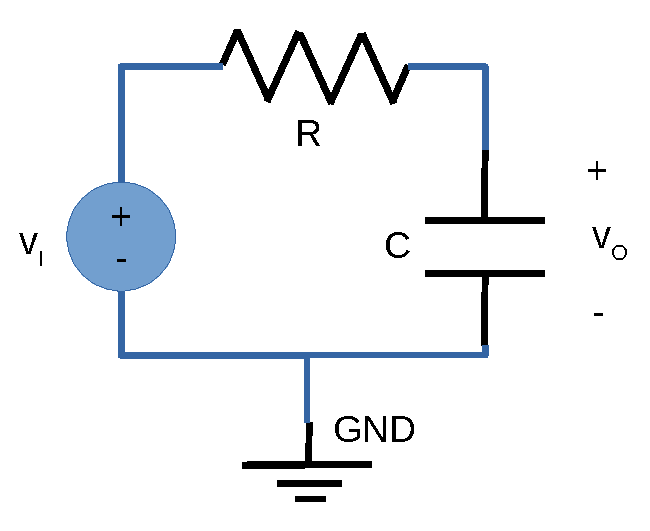
\includegraphics[width=0.7\linewidth]{rc.pdf}
\caption{Given circuit.}
\label{fig:rc}
\end{figure}




\section{Theoretical Analysis}
\label{sec:analysis}

In this section, the circuit shown in Figure~\ref{fig:t1_circuit} is analysed
theoretically using the mesh method and the node method.

\subsection{Mesh Method}

To determine all the currents of a planner circuit, they can be replaced by fictitious currents and, subsequently, the Mesh Method based on Kirchhoff's Voltage Law and Ohm's Law can be applied.\par

\begin{figure}[h] \centering
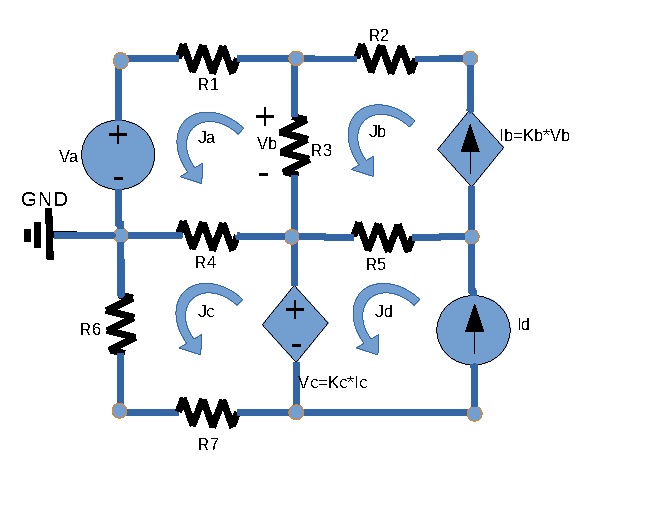
\includegraphics[width=0.55\linewidth]{t1_circuit_MM.pdf}
\caption{Circuit with mesh currents (Mesh Method).}
\label{fig:t1_circuit_MM}
\end{figure}


\par
According to this method, the algebraic sum of voltages around a loop equals zero or, in other way, the sum of voltage rises equals the sum of voltage drops around a loop. Applying this method the only unknown variables are the currents that circulate on each mesh. So, for mesh A:
\begin{equation}
  J_a\times R_1 + V_a + R_4\times (J_a - J_c) + R_3\times (J_a - J_b) = 0
  \label{eq:kvl}
\end{equation}

Mesh B:
\begin {equation}
  J_b = I_b = K_b\times V_b = K_b\times R_3\times (J_b - J_a)
  \label {eq:kvl}
\end{equation}

Mesh C:
\begin {equation}
  J_c\times R_7 - K_c\times J_c + R_4\times (J_c - J_a) + R_6\times J_c = 0
  \label {eq:kvl}
\end{equation}

And mesh D:
\begin {equation}
  J_d = I_d
  \label {eq:kvl}
\end{equation}
 
 By computing this four equations in function of the four variables: Ja, Jb, Jc e Jd. The values presented in Table~\ref{tab:MM} were obtained. For this calculations it was used the mathematical tool, Octave.

\begin{table}[h]
  \centering
  \begin{tabular}{|l|r|}
    \hline    
    {\bf Name} & {\bf Value [A]} \\ \hline
    Ja & -0.00022595\\ \hline
Jb & -0.00023645\\ \hline
Jc &  0.00095088\\ \hline
Jd &  0.0010264\\ \hline

  \end{tabular}
  \caption{Theoretical values obtained using octave to solve equations of mesh method.}
  \label{tab:MM}
\end{table}


\subsection{Node Method}

\begin{figure}[h] \centering
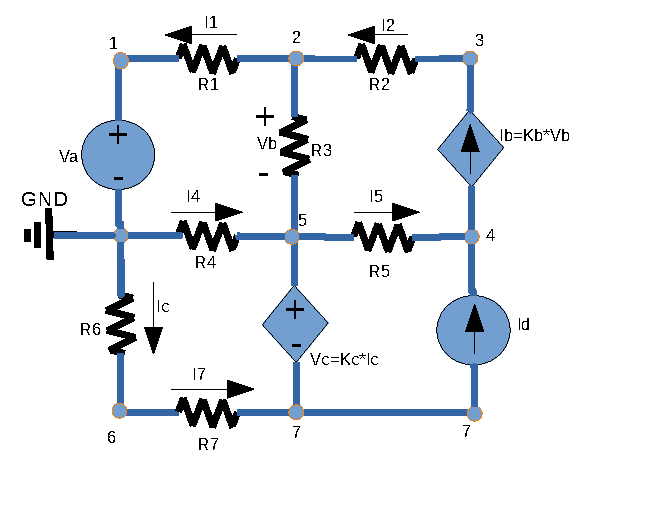
\includegraphics[width=0.6\linewidth]{t1_circuit_NM.pdf}
\caption{Circuit with currents and nodes identified (Node Method).}
\label{fig:t1_circuit_NM}
\end{figure}

In the same way, we can apply the node method, this method is based in the Kirchhoff's Current Law (KCL) and in the Ohm's Law, to analyse circuits. According to this method, KCL is applied in nodes that aren't connected to voltage sources and the currents flowing into a node must add up to zero, which means that the algebraic sum of currents that enters into a node equals to the algebraic sum of currents that exits that node. In nodes related by voltage sources, additional equations are applied. 
So, applying KCL for node 2, we have:
\begin {equation}
  (V_3 - V_2)\times G_2 = (V_2 - V_1)\times G_1 + (V_2 - V_5)\times G_3
  \label {eq:kvl}
\end{equation}

Node 3:
\begin{equation}
(V_3- V_2)\times G_2 = K_b\times (V_2 - V_5)
  \label {eq:kvl}
\end{equation}

Node 4:
\begin {equation}
I_d + (V_5 - V_4)\times G_5 = K_b\times (V_2 - V_5)
  \label {eq:kvl}
\end{equation}

And node 6:
\begin {equation}
(-V_5)\times G_6 = (V_6 - V_7)\times G_7
  \label {eq:kvl}
\end{equation}

The additional equations are:

\begin {equation}
V_1= V_a
  \label {eq:kvl}
\end{equation}

\begin {equation}
V_5 - V_1 = K_c\times (-V_6)\times G_6
  \label {eq:kvl}
\end{equation}

\begin {equation}
(V_6 - V_7)\times G_7 + (-V_5)\times G_4 + (V_2 - V_5)\times G_3 = (V_5 - V_4)\times G_5 + I_D
  \label {eq:kvl}
\end{equation}

The equations (9) and (10) are obtained using the voltage drop between the two voltage sources. The last equation was derived using a super-node that contains the dependent voltage source. Applying the node law, the sum of currents that enter the dependent voltage source is equal to the sum of currents that leaves it. 

\begin{table}[h]
  \centering
  \begin{tabular}{|l|r|}
    \hline    
    {\bf Name} & {\bf Value [A or V]} \\ \hline
    V0 & 0\\ \hline
V1 &  5.0102\\ \hline
V2 &  4.7774\\ \hline
V3 &  4.2972\\ \hline
V4 &  8.6049\\ \hline
V5 &  4.8099\\ \hline
V6 & -1.9313\\ \hline
V7 & -2.9274\\ \hline

  \end{tabular}
  \caption{Theoretical values obtained using octave to solve equations of Node Method.}
  \label{tab:NM}
\end{table}







\section{Simulation Analysis}
\label{sec:simulation}


\subsection{Operating Point Analysis for t\textless0}

Table~\ref{tab:op1} shows the simulated operating point results for the circuit
under analysis. Compared to the theoretical analysis results, we can see that the values are exactly the same.

\begin{table}[ht]
  \centering
  \begin{tabular}{|l|r|}
    \hline    
    {\bf Name} & {\bf Value [A or V]} \\ \hline
    \input{values1_tab}
  \end{tabular}
  \caption{Operating point. A variable preceded by @ is of type {\em current}
    and expressed in Ampere; other variables are of type {\it voltage} and expressed in
    Volt.}
  \label{tab:op1}
\end{table}



\subsection{Operating Point Analysis for vs(t)=0}

Table~\ref{tab:op2} shows the simulated operating point results for the circuit, this time with the null voltage source and with the replacement of the capacitor by a voltage source $V_x=V(6)-V(8)$. This procedure is necessary to determine the initial conditions, in this case they correspond to the ones of a saturated capacitor. 

\begin{table}[ht]
  \centering
  \begin{tabular}{|l|r|}
    \hline    
    {\bf Name} & {\bf Value [A or V]} \\ \hline
    \input{values2_tab}
  \end{tabular}
  \caption{Operating point. A variable preceded by @ is of type {\em current}
    and expressed in Ampere; other variables are of type {\it voltage} and expressed in
    Volt.}
  \label{tab:op2}
\end{table}

\newpage

\subsection{Simulation of the natural response of the circuit}

In this point we have simulated the natural response of the circuit, using the boundary conditions V(6) and V(8) as obtained in 3.2). Then we used Ngspice’s transient analysis mode to get v6(t) in the interval [0, 20] ms. Finally we have plotted the result, as you can see in Figure 10. This plot is equal to the one get in the theoretical analyses
\vspace{-0.9in}
\begin{figure}[H] \centering
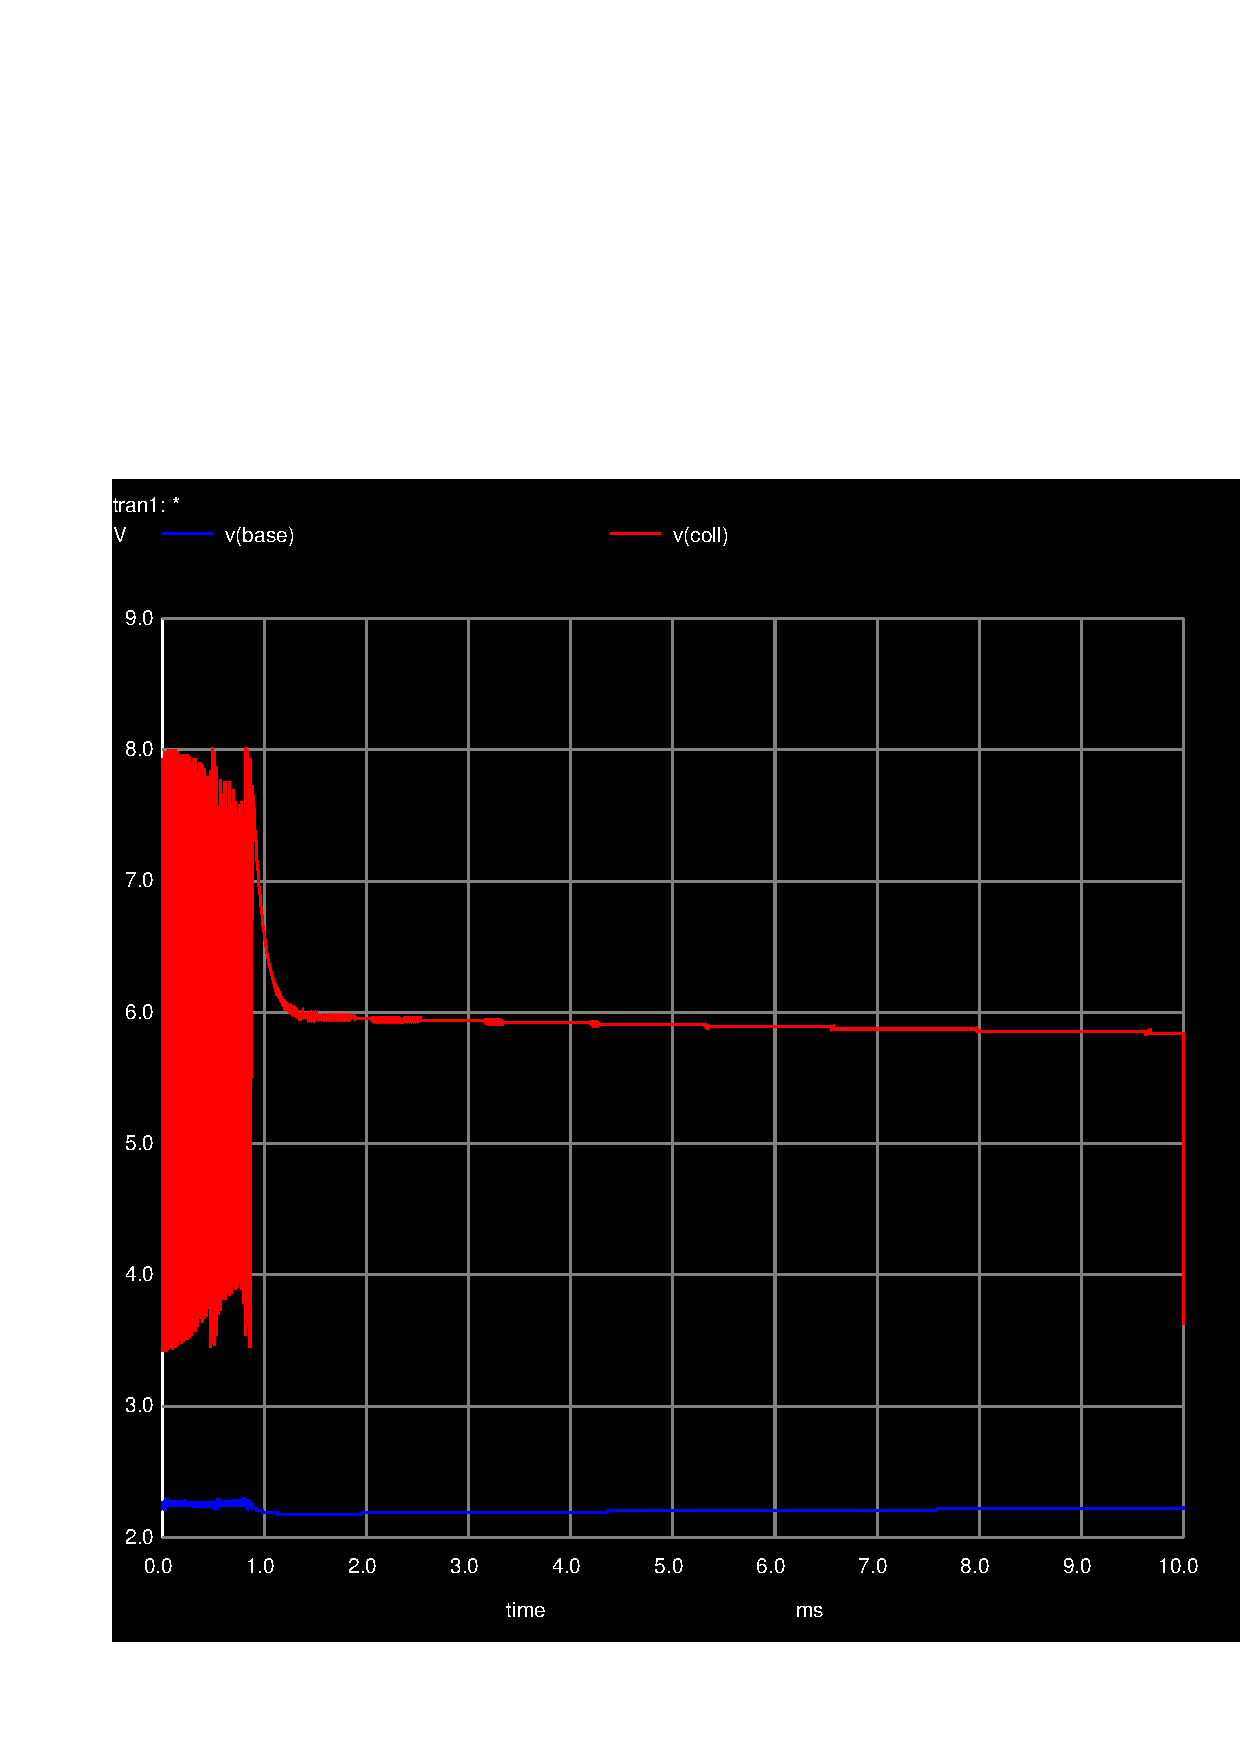
\includegraphics[width=0.45\linewidth]{trans.pdf}
\caption{Transient natural response output of voltage V6}
\label{fig:trans}
\end{figure}



\subsection{Simulation of the natural and forced response of the circuit}


We simulated the natural and forced response on node 6 by repeating step  3) (3.3) with $v_s(t)$ as given in Fig. 1 and with f=1kHz. Then we plotted both the stimulus and the response.
\vspace{-1.2in}
\begin{figure}[H] \centering
\includegraphics[width=0.45\linewidth]{trans2.pdf}
\caption{Transient total response output voltage V6}
\label{fig:trans2}
\end{figure}



\subsection{Simulation of the frequency response in node 6 } 

The next point was to do the response in frequency, as it was already referred, the increase in frequency, decreases the capacitor impedance, this is, the tension will decrease. This is the reason why we observe a negative variation in terms of magnitude in the Bode's diagram, since 10Hz to $10^4$ Hz. With the influence of this frequency the variation on the capacitor is so small, that is not going to interfere with v6. As Vs is a voltage source both its magnitude and phase do not change.

\vspace{-0.9in}

\begin{figure}[H] \centering
\includegraphics[width=0.45\linewidth]{acmag.pdf}
\caption{Frequency response (Bode Diagram: Magnitude)}
\label{fig:acmag}
\end{figure}

\vspace{-1in}

\begin{figure}[H] \centering
\includegraphics[width=0.45\linewidth]{acphase.pdf}
\caption{Frequency response (Bode Diagram: Phase)}
\label{fig:acphase}
\end{figure}

\newpage






\section{Conclusion}
\label{sec:conclusion}

In this laboratory assignment the objective of analysing an RC circuit has been
achieved. Static, time and frequency analyses have been performed both
theoretically using the Octave maths tool and by circuit simulation using the
Ngspice tool. The simulation results matched the theoretical results
precisely. The reason for this perfect match is the fact that this is a
straightforward circuit containing only linear components, so the theoretical
and simulation models cannot differ. For more complex components, the
theoretical and simulation models could differ but this is not the case in this
work.





%\cleardoublepage

% ----------------------------------------------------------------------
%  Bibliography
% ----------------------------------------------------------------------
%\addcontentsline{toc}{section}{\bibname}
%\bibliographystyle{abbrvunsrtnat} % <<<<< SELECT IF USING REFERENCES BY NUMBER (CITATION ORDER)
%\bibliography{../../../BIBfile.bib}

% ----------------------------------------------------------------------
\end{document}
% ----------------------------------------------------------------------

